\documentclass[document.tex]{subfiles} 
\begin{document}
\section{Аппаратное обеспечение}
\subsection{Акселерометр}
\subsubsection{Описание и сравнение акселерометров}
Акселерометр может применяться как для измерения проекций абсолютного линейного
ускорения, так и для косвенных~(через силу реакции опоры) измерений проекции
гравитаци\-онного ускорения.

Первое свойство используется для создания инерциальных навигационных систем, где
полученные с помощью акселерометров измерения интегрируют, получая
инерци\-альную ско\-рость и координаты носителя. Таким образом, акселерометры, наравне с
гироско\-пами, являются неотъемлемыми компонентами систем навигации и управления
самолётов, ракет и других летательных аппаратов, кораблей и подводных лодок.
Второе свойство позволяет использовать акселерометры для измерения уклонов, то
есть в качестве инклино\-метров.\cite{accelerometer_info}

Используя акселерометр в качестве инклинометра, то есть прибора,
предназначенного для измерения величины и азимута угла наклона различных
объектов относительно гравита\-ционного поля Земли, можно реализовать функционал,
характерный для уровней.

Между цифровыми и аналоговыми акселерометрами, следует выбрать цифровые, так
как они не требуют внешних компонентов, и не требуют никаких расчётов: все их
метро\-логические характеристики указаны. Стоить они будут дороже аналоговых, но
время, затра\-чиваемое на разработку системы
снижается.\cite{accelerometer_compare}

Общие сравнительные характеристики цифровых акселерометров указаны в таблице~\ref{tabular:accelerometer_compare_common}.

\begin{table}[h]
\medskip
\resizebox{\linewidth}{!}{
\tabcolsep=2pt
\begin{tabular}{|c|c|c|c|c|c|c|c|c|}
\hline
Модель&Кол-во осей&Напряжение питания&Интерфейс&
Пределы измерений&Частота выборки, Гц&Погр-ть
нуля, mg&Разрешение, mg\\
\hline
MMA7450		&3		&2.4 -- 3.6~В	&I\textsuperscript{2}C, SPI	&\pm2g, \pm4g, \pm8g			&125, 250	&250	&15.6 \\
MMA7660		&3		&2.4 -- 3.6~В	&I\textsuperscript{2}C		&\pm1.5g						&1 -- 120	&64		&21.33 \\
MMA7455		&3		&2.4 -- 3.6~В	&I\textsuperscript{2}C, SPI	&\pm2g, \pm4g, \pm8g			&125, 250	&330	&15.6 \\
ADXL345		&3		&2.0 -- 3.6~В	&I\textsuperscript{2}C, SPI	&\pm2g, \pm4g, \pm8g, \pm16g	&0.1 -- 3200&150	&3.9 \\
SMB380		&3		&2.4 -- 3.6~В	&I\textsuperscript{2}C, SPI	&\pm2g, \pm4g, \pm8g			&25 -- 1500	&60		&4 \\
LIS202DL	&2		&2.2 -- 3.6~В	&I\textsuperscript{2}C, SPI	&\pm2g, \pm8g					&100, 400	&40		&18 \\
LSM303DLM	&3 + 3	&2.16 -- 3.6~В	&I\textsuperscript{2}C		&\pm2g, \pm4g, \pm8g			&			&60		&1 \\
\hline
\end{tabular}}
\medskip
\caption{Общие характеристики цифровых акселерометров}
\label{tabular:accelerometer_compare_common}
\end{table}

\clearpage
\subsubsection{Характеристики акселерометра MMA7660}
Неплохим выбором, исходя из таблицы~\ref{tabular:accelerometer_compare_common}, является MMA7660 компании Freescale Semiconductor, имеющий следующие технические характеристики:
\begin{itemize}
	\item цифровой вывод (I\textsuperscript{2}C);
	\item 3mm x 3mm x 0.9mm DFN-чип; 
	\item низкое энергопотребление;
	\item настраиваемую частоту снятия показаний от 1 до 120 в секунду;
	\item низкий вольтаж (2.4 В -- 3.6 В~--- аналоговый; 1.71 В -- 3.6 В~--- цифровой);
	\item автоматический режим сна для уменьшения энергопотребления;
	\item определение ориентации в пространстве;
	\item совместимость с RoHS;
	\item отсутствие галогенов;
	\item низкую цену.
\end{itemize}

\noindent
Примеры типового применения акселерометра MMA7660, согласно документации, следующие:
\begin{itemize} 
	\item мобильные телефоны/ PMP/PDA: оперделение ориентации (портретная/пейзажная), стабилизация изображения, прокрутка текста, звонок по встряхиванию;
	\item настольные компьютеры: защита от кражи;
	\item игры: определение движения, автоматический режим сна для уменьшения энерго\-потребления;
	\item цифровые камеры: стабилизация изображения. \cite{accelerometer_mma7660}
\end{itemize}

\clearpage
\subsubsection{Устройство акселерометра MMA7660}
Цоколевка и функциональное устройство акселерометра MMA7660 представлены на ри\-сунке~\ref{fig:mma7660fc_pinout_scheme}.

\begin{figure}[here]
\centering
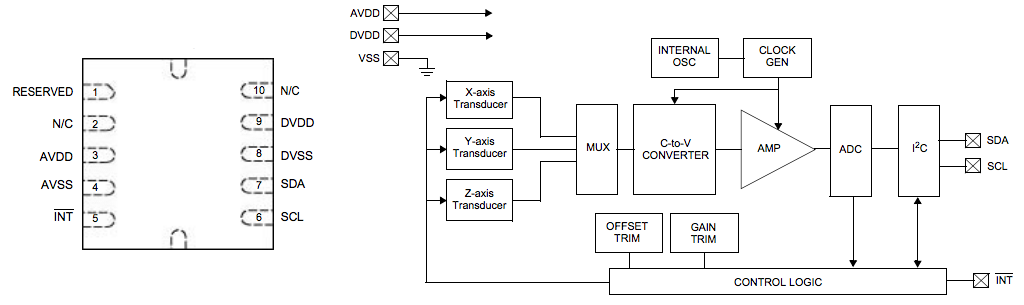
\includegraphics[width=1\linewidth]{mma7660fc_pinout_scheme}
\caption{Цоколевка и функциональное устройство акселерометра MMA7660}
\label{fig:mma7660fc_pinout_scheme}
\end{figure}

В таблице~\ref{tabular:mma7660fc_scheme} представлено описание выходов и выходов акселерометра MMA7660. 

\begin{table}[h]
\medskip
\resizebox{\linewidth}{!}{
\tabcolsep=2pt
\begin{tabular}{|c|c|c|c|c|c|c|c|c|}
\hline
Номер ножки&Наименование&Описание&Статус \\
\hline
1 	&RESERVED 	&Подключается к AVSS						&Вход \\
2 	&N/C 		&Без соединения, подключается к заземлению	&Вход \\
3 	&AVDD 		&Питание устройства							&Вход \\
4 	&AVSS 		&Заземление устройства						&Вход \\
5 	&INT 		&Прерывание/готовность данных				&Выход \\
6 	&SCL 		&Тактовые импульсы I\textsuperscript{2}C		&Вход \\
7 	&SDA 		&Последовательные данные I\textsuperscript{2}C&Открытый коллектор \\
8 	&DVSS 		&Цифровое заземление I/O					&Вход \\
9 	&DVDD 		&Цифровое питание I/O						&Вход \\
10 	&N/C 		&Без соединения, подключается к заземлению	&Вход \\
\hline
\end{tabular}}
\medskip
\caption{Общие характеристики цифровых акселерометров}
\label{tabular:mma7660fc_scheme}
\end{table}

\clearpage
\subsubsection{Подключение акселерометра MMA7660 к микроконтроллеру}
Акселерометр MMA7660 подключается к микроконтроллеру с использованием протокола I\textsuperscript{2}C. Схема подключения представлена на рисунке~\ref{fig:mma7660fc_connection}.

\begin{figure}[here]
\centering
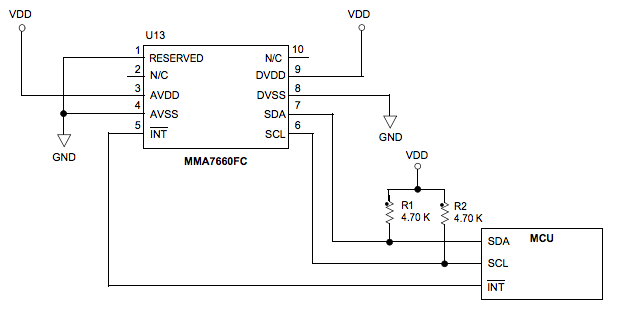
\includegraphics[width=0.7\linewidth]{mma7660fc_connection}
\caption{Цоколевка и функциональное устройство акселерометра MMA7660}
\label{fig:mma7660fc_connection}
\end{figure}

Входы AVDD и DVDD подключаются к источнику питания, входы AVSS и DVSS (опцио\-нально, входы N/C) подключаются к заземлению, выход INT подключается к микрокон\-троллеру
напрямую, а контакты SCL и SDA из-за использования открытых коллекторов, подключаются с использованием подтягивающих резисторов на 4.7 кОм.\cite{accelerometer_mma7660, basics}

\clearpage
\subsubsection{Тайминги акселерометра MMA7660}
На рисунке~\ref{fig:mma7660fc_timing_common} показан общий тайминг протокола I\textsuperscript{2}C, используемого акселерометром для передачи и приема данных с микроконтроллера.
\begin{figure}[here]
\centering
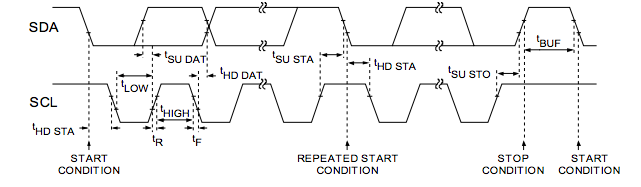
\includegraphics[width=0.8\linewidth]{mma7660fc_timing_common}
\caption{Общий тайминг протокола I\textsuperscript{2}C акселерометра MMA7660}
\label{fig:mma7660fc_timing_common}
\end{figure}

Подтверждающим битом передачи байта является 9-й бит. Подтверждающий бит выстав\-ляется низким уровнем сигнала акселерометра для подтверждения приема байта на открытом коллекторе
SDA. При этом на самом микроконтроллере выставляется высокий уровень. Тайминг передачи байта и подтверждения передачи приведен на
рисунке~\ref{fig:mma7660fc_timing_byte}.\cite{accelerometer_mma7660}

\begin{figure}[here]
\centering
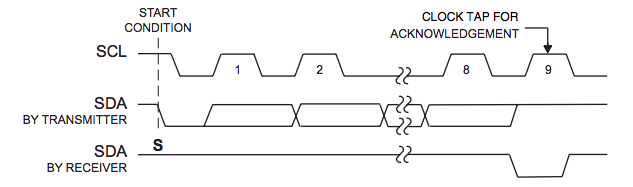
\includegraphics[width=0.8\linewidth]{mma7660fc_timing_byte}
\caption{Общий тайминг протокола I\textsuperscript{2}C акселерометра MMA7660}
\label{fig:mma7660fc_timing_byte}
\end{figure}

\clearpage
\subsection{Дисплей}
\subsubsection{Общие характеристики дисплея LCD-NHD-C12832A1Z}
В качестве устройства вывода для отображения отклонения от горизонтали, решено выбрать дисплей LCD-NHD-C12832A1Z, имеющий следующие технические характеристики:
\begin{itemize}
	\item 128 x 32 пикселей;
	\item 4-канальный интерфейс SPI;
	\item встроенный контроллер ST7565R;
	\item вольтаж +3.0В;
	\item скважность 33; диапазон рабочих напряжений 1/6;
	\item совместимость с RoHS.\cite{display}
\end{itemize}
\subsubsection{Схема подключения дисплея LCD-NHD-C12832A1Z к микроконтроллеру}
Дисплей LCD-NHD-C12832A1Z подключается к микроконтроллеру с использованием про\-токола SPI с четырьмя каналами. Схема подключения представлена на
рисунке~\ref{fig:display_connection}. Помимо входа источника питания VDD и входа заземления VSS, входов питания для подключения конденсаторов, также присутствует вход питания A и
вход заземления K для подсветки дисплея, вход сброса /RST. Для интерфейса SPI предусмотрены входы /CS1 (Chip Select), SCL (Serial Clock), SI (Master Output, Slave Input), а также
канал выбора регистра инструкций или данных A0.\cite{display, lcd_interfaces}

\begin{figure}[here]
\centering
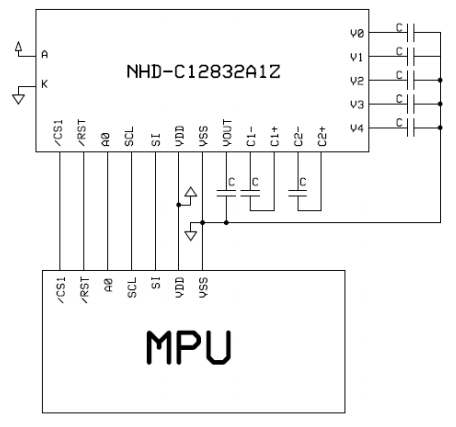
\includegraphics[width=0.6\linewidth]{display_connection}
\caption{Схема подключения дисплея LCD-NHD-C12832A1Z к микроконтроллеру}
\label{fig:display_connection}
\end{figure}

\clearpage
\subsubsection{Тайминги дисплея LCD-NHD-C12832A1Z}
На рисунке~\ref{fig:display_timing} показан общий тайминг 4-канального протокола SPI, используемого дисплеем для приема данных с микроконтроллера.
\begin{figure}[here]
\centering
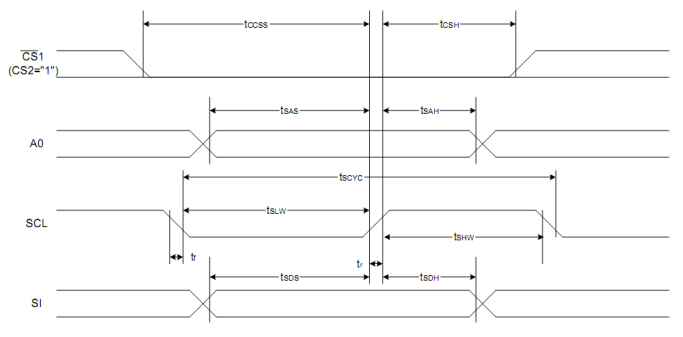
\includegraphics[width=0.8\linewidth]{display_timing}
\caption{Общий тайминг протокола SPI дисплея LCD-NHD-C12832A1Z}
\label{fig:display_timing}
\end{figure}

На рисунке~\ref{fig:display_timing_reset} приведен тайминг сброса дисплея LCD-NHD-C12832A1Z.
\begin{figure}[here]
\centering
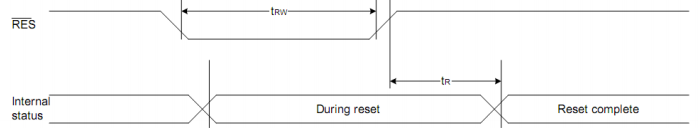
\includegraphics[width=0.8\linewidth]{display_timing_reset}
\caption{Тайминг сброса дисплея LCD-NHD-C12832A1Z}
\label{fig:display_timing_reset}
\end{figure}

\clearpage
\subsection{Микроконтроллер}
\subsubsection{Общие характеристики микроконтроллера STM32F405RGT6}
В качестве микроконтроллера решено выбрать STM32F405RGT6, имеющий следующие технические характеристики:
\begin{itemize}
	\item Ядро: ARM 32-bit Cortex™-M4 CPU с FPU,
адаптивный акселератор реального времени (ART
Accelerator™), позволяющий выполнять инструкции с Flash без задержек, частота до 168 МГц,
модуль защиты памяти, 210 DMIPS/ 1.25 DMIPS/МГц (Dhrystone 2.1) и инструкциями DSP
	\item Память
	\begin{itemize}
		\item До 1 Мб Flash-памяти
		\item До 192+4 Кб SRAM, включая 64 Кб CCM (кэш процессора) оперативная память данных
		\item Контроллер памяти, поддерживающий Compact Flash, SRAM, PSRAM, NOR и NAND
	\end{itemize}
	\item Параллельный интерфейс LCD 8080/6800
	\item Управление тактированием, перезагрузкой, цепями
	\begin{itemize}
		\item Питание I/O от 1.8 В до 3.6 В
		\item POR, PDR, PVD и BOR
		\item Поддержка кварцевого генератора от 4 до 26 МГц
		\item Внутренний 16 МГц кварцевого генератора (1\% точность)
		\item 32 кГц генератор сигналов для RTC с калибровкой
		\item Внутренний 32 kHz кварцевого генератор с калибровкой
	\end{itemize}
	\item Пониженное питание
	\begin{itemize}
		\item Спящий режим, режим останова и режим простоя
		\item VBAT питание для RTC, 20 x 32-битных запасных регистров + дополнительные 4 Кб запасной SRAM
	\end{itemize}
	\item 3 x 12-битных 2.4 MSPS A/D конвертера: до 24 каналов и 7.2 MSPS в тройном режиме чередования
	\item 2 x 12-битных D/A конвертера 
	\item DMA общего назначения: 16-поточный контроллер DMA с FIFO и пакетной поддержкой
	\item До 17 таймеров: до 12 x 16-битных и двух 32-битных таймеров до 168 МГц, каждый может иметь до 4
IC/OC/PWM или вход счетчика импульсов и квадратурного (инкре\-ментального) кодера
	\item Отладочный режим
	\begin{itemize}
		\item Интерфейсы последовательной отладки (SWD) и JTAG
		\item Cortex-M4 Embedded Trace Macrocell™
	\end{itemize}
	\item До 140 портов ввода / вывода с возможностью прерываний
	\begin{itemize}
		\item До 136 быстрых портов I/O частотой до 84 МГц
		\item До 138 портов I/O с поддержкой 5 В
	\end{itemize}
	\item До 15 интерфейсов передачи данных
	\begin{itemize}
		\item До 3 x I\textsuperscript{2}C интерфейсов (SMBus/PMBus)
		\item До 4 интерфейсов USART / 2 UART (10.5 Мбод, интерфейс ISO 7816, LIN, IrDA, управление модемом)
		\item До 3 интерфейсов SPI (42 Мбод) с двумя полнодуплексными интерфейсами I2S для достижения высокой точности аудио с использованием внутренней фазовой автоподстройки частоты
		или внешнего генератора
		\item 2 x интерфейса CAN (активные 2.0B)
		\item интерфейс SDIO
	\end{itemize}
	\item Дополнительные интерфейсы передачи данных
	\begin{itemize}
		\item USB 2.0 полноскоростной device/host/OTG
контроллер с PHY на кристалле
		\item USB 2.0 высокоскоростной/полноскоростной
device/host/OTG контроллер с выде\-ленной DMA, полноскоростной PHY на кристалле и ULPI
		\item 10/100 Ethernet MAC с выделенной DMA:
поддержка IEEE 1588v2, MII/RMII
	\end{itemize}
	\item От 8 до 14-битный параллельный интерфейс камеры до 54 Мбайт/c
	\item Генератор случайных чисел TRNG
	\item Модуль вычислений контрольных сумм
	\item Уникальный 96-битный идентификатор
	\item RTC: субсекундная точность, аппаратный календарь\cite{mcu}
\end{itemize}
\end{document}
